\documentclass[12pt,a4paper]{article}
\usepackage[utf8]{inputenc}
\usepackage[russian]{babel}
\usepackage[left=2.00cm, right=2.00cm, top=2.00cm, bottom=2.00cm]{geometry}
\linespread{1.25}
\usepackage{setspace}
\usepackage{indentfirst}
\setlength{\parindent}{1.25cm}
\let\paragraph\ignorespaces
\usepackage{tabularx}
\usepackage{multirow}
\usepackage{graphicx}



\begin{document}
	
\begin{titlepage}
	
\begin{center}
	\large Университет ИТМО\\[5cm]
	\LARGE Практическая работа №3\\
	\normalsize по дисциплине <<Визуализация и моделирование>>\\[5cm]
\end{center}
\begin{flushright}
		\begin{minipage}{0.6\textwidth}
		\begin{flushleft}
			\large
			\singlespacing 
			\textbf{Автор:} Костылев Иван Михайлович\\
			\textbf{Поток:} 1.1\\
			\textbf{Группа:} K3240\\
			\textbf{Факультет:} ИКТ\\
			\textbf{Преподаватель:} Чернышева А.В.
		\end{flushleft}
	\end{minipage}
\end{flushright}

\vfill

\begin{center}
	{\large Санкт-Петербург, \the\year{ г.}}
\end{center}
 
\end{titlepage}
\normalsize


\large \textbf{Описание датасета}

\normalsize
	Датасет состоит из данных о студентах, их родителей и оценок, полученных ими по различным предметам. \\

Всего записей: 1000 \\


\large \textbf{Формальное описание}

\begin{tabular}{ | p{100pt} | p{100pt} | p{100pt} | p{40pt} | p{60pt} |}
\hline
Столбец & Описание & Значения & Формат & Шкала  \\ \hline
gender & пол студента & male / female & текст & Качеств номинальная \\ \hline
race/ethnicity & расовая классификация & group A / group B / group C / group D & текст & Качеств номинальная  \\ \hline
parental level of education & уровень образования родителей & collegue / school / bachelor's degree / others  & текст & Качеств номинальная  \\ \hline
lunch & оплата обеда & standart / free/reduced & текст & Качеств номинальная  \\ \hline
test preparation & подготовка к тесту & none / completed & текст & Качеств номинальная  \\ \hline
math score & оценка по математике & 0..100 & целое число & Колич относительная  \\ \hline
reading score & оценка по чтению & 0..100 & целое число & Колич относительная  \\ \hline
writting score & оценка по письму & 0..100 & целое число & Колич относительная  \\ \hline
\end{tabular}
\\
\\

\large \textbf{Описание проблем}

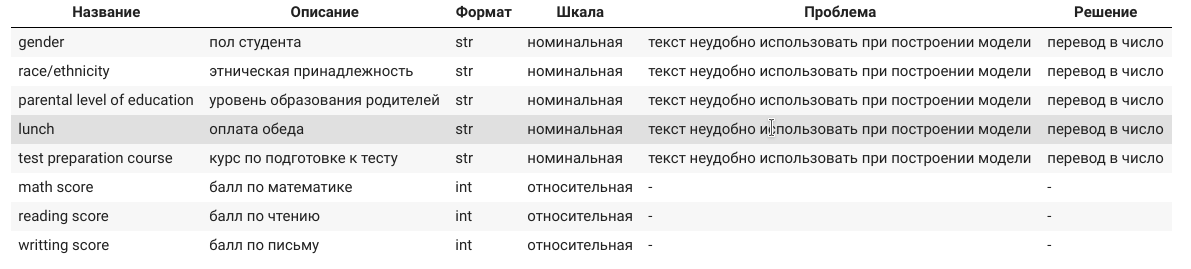
\includegraphics[scale=0.5]{table}


\newpage
\large \textbf{Подготовка данных}

\textit{Полный код лежит в блокноте: 
\\ https://colab.research.google.com/drive/1V56fg3-hLgE9BnUmFQGEiFc8l21EHF0e?usp=sharing}\\

\textbf{1. Обработка пустых ячеек.} \\
В датасете отсутствуют пустые ячейки. Убеждаемся в этом:

\begin{verbatim}
df.isnull().sum()
\end{verbatim}

Output:
\begin{verbatim}
gender                         0
race/ethnicity                 0
parental level of education    0
lunch                          0
test preparation course        0
math score                     0
reading score                  0
writing score                  0
dtype: int64
\end{verbatim}

\textbf{2. Для построения моделей данных в следующих работах нам необходимо перевести текст в числовые значения.}

1) Столбец 'gender' (male / female): \\
Категориальный признак.
Нормализуем его с помощью следующей функции:

\begin{verbatim}
def norm_gender(gender: str) -> int:
  if gender == 'male':
    return 0
  else:
    return 1
\end{verbatim}

Значению 'male' соответствует 0, 'female' - 1.

\begin{verbatim}
PREP = 'test preparation course'
df_norm = df.copy()
df_norm[PREP] = df_norm[PREP].apply(norm_preparation)
\end{verbatim}


\textbf{2) Столбец 'test preparation course'} (none / completed): \\
Категориальный признак.
Нормализуем его с помощью следующей функции:

\begin{verbatim}
def norm_preparation(is_prepared: str) -> int:
  if is_prepared == 'none':
    return 0
  else:
    return 1
\end{verbatim}

Таким образом, значению 'none' (не проходил курс) будет соответствовать 0, 'completed' - 1.

\begin{verbatim}
PREP = 'test preparation course'
df_norm = df.copy()
df_norm[PREP] = df_norm[PREP].apply(norm_preparation)
\end{verbatim}

\textit{Нормализация остальных данных выполнялась аналогичным способом, поскольку они также являются категориальными (кроме столбцов с оценками).}\\

\textbf{Гипотезы}\\
Опираясь только лишь на описательную статистику из лаборатнорной работы №2, на данном этапе сложно построить новые гипотезы.

Хотелось бы ещё узнать немного о самом датасете, поэтому сформулируем следующие вопросы:

1. Кто лучше справлялся с задачами по предметам - мужчины или женщины?

\begin{verbatim}
width = 0.3
genders = ['male', 'female']
x = np.arange(len(genders))
scores = [sum(male_score.values())/3, sum(female_score.values())/3]
fig, ax = plt.subplots()
graph = ax.bar(x, scores, width, label='Score')
ax.set_title('Распределение оценок у мужчин и женщин')
ax.set_xticks(x)
ax.set_xticklabels(genders)
ax.legend()
\end{verbatim}

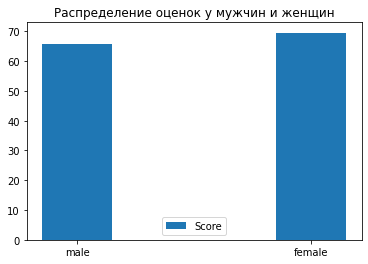
\includegraphics{mf_score_avg}

Если брать средние баллы, то видно, что женщины справляются с задачами лучше.\\
\textit{Детализируем по предметам вопрос:}

\textbf{2. Кто как из мужчин/женщин справлялся с задачами по каждому предмету в отдельности?}

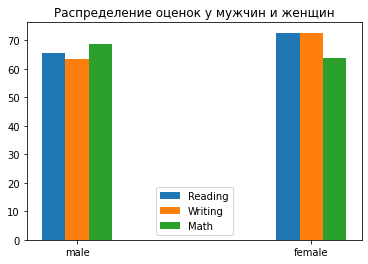
\includegraphics{mf_score}

\textit{Проведем похожее исследование по поиску зависимостей между категориальными данными и числовыми}
\\
\\
\textbf{3. Гипотеза: чем выше уровень образования у родителей, тем выше средний балл студента}


\begin{verbatim}
import statistics as stat

middle_score_list
df['avg_score'] = middle_score_list
parental_levels = df[PLE].unique()
level_scores = {}
scores_only = []
for level in parental_levels:  
  level_scores[level] = stat.mean(list(df[df[PLE] == level]['avg_score']))
  scores_only.append(level_scores[level])

x = np.arange(len(parental_levels))
fig, ax = plt.subplots()
graph = ax.bar(x, scores_only, width, label='Score')

ax.set_title('Зависимость уровня сдачи экзамена от образования родителей')
ax.set_xticks(x)
ax.set_xticklabels(parental_levels, rotation = 'vertical')
ax.legend()

\end{verbatim}

Из рисунка ниже видно, что самые большие баллы получили дети родителей с высшим образованием. Ранжирование уровня сдачи можно сопоставить уровню образования родителей.

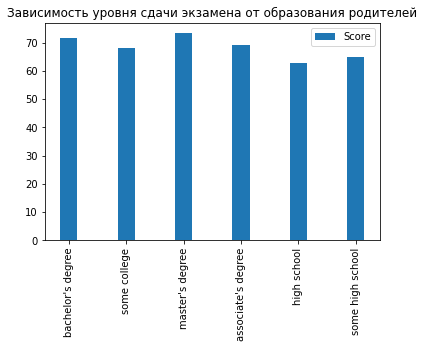
\includegraphics{parental_degree_score}

\textbf{4. Гипотеза: баллы по математике плохо коррелируются с баллами по чтению и письму}
\\
\textbf{5. Гипотеза: баллы по письму и чтению коррелируются лучше между собой и со средним значением}

Построим матрицу корреляции:\\
На ней\\
0 - математика\\
1 - чтение\\
2 - письмо\\
3 - среднее значение\\
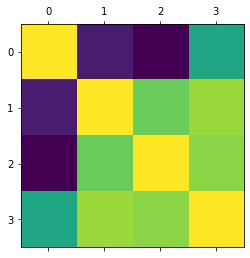
\includegraphics{corr}

Наши гипотезы 4 и 5 подтвердились частично:\\
Гипотеза (4) верна. Отсюда может следовать вывод о разделении людей на гуманитариев и технарей (т.к. видно, что оценки по гуманитарным предметам и математике коррелируются не так хорошо).\\
Гипотеза (5) подтвердилась частично. Письмо и чтение действительно коррелируют друг с другом, однако в сравнении со средним значением у них разброс достаточно большой.

\end{document}